\begin{figure}[t]
\centering
    \begin{subfigure}[t]{0.45\textwidth}
    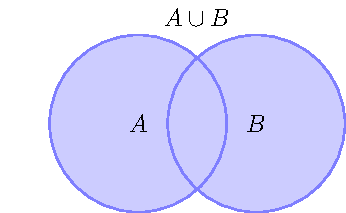
\includegraphics[width=\textwidth]{figures/math/set_theory/set_venn_or.pdf}
    \end{subfigure}
    \begin{subfigure}[t]{0.45\textwidth}
    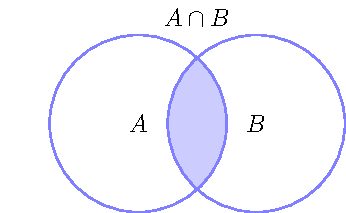
\includegraphics[width=\textwidth]{figures/math/set_theory/set_venn_and.pdf}
    \end{subfigure}

    \begin{subfigure}[t]{0.45\textwidth}
    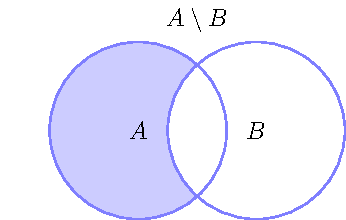
\includegraphics[width=\textwidth]{figures/math/set_theory/set_venn_minus.pdf}
    \end{subfigure}
    \caption[Set operations]{Here is a figure of various set operations:
        set union, set intersection, and set minus.
        Modified from an example online~\cite{vennDiagram}.}
    \label{fig:math_set_venn}
\end{figure}
